\documentclass[11pt]{article}
\usepackage[margin=1in]{geometry}
\usepackage{amsmath, amssymb, amsthm, esint}
\usepackage{fancyhdr}
\usepackage{tikz, tikz-3dplot}
% \usepackage{hyperref}
\usepackage{cancel}
\usetikzlibrary{spy}

\setlength{\headheight}{14pt}
\fancyhf{}
\lhead{Single Variable Calculus: Derivative}
\cfoot{\thepage}

\begin{document}
\pagestyle{plain}
\begin{center}
  \tableofcontents
\end{center}
\newpage
\setcounter{page}{1}
\pagestyle{fancy}

\section{Definition and The First Principle}
\subsection{Definition}
Let $f$ be a function defined on an open interval containing $a$.  
The \textbf{derivative} of $f$ at the point $a$, denoted by $f'(a)$, is defined as
\begin{align*}
    f'(x)\,&=\lim_{h \to 0} \frac{f(x + h)-f(x)}{h}\\
        &=\lim_{x \to a}\frac{f(x)-f(a)}{x-a}
\end{align*}
\subsection{The derivative at a Point $a$}
\[
    f'(a)=\lim_{h\to 0}\frac{f(a+h)-f(a)}{h}
\]
provided the limit exists.
\subsection{Geometric Meaning}
To find the slope of the tangent line to the curve $y = f(x)$ at a point $x = a$, we consider the slope of the secant line between two points:
\[
    \frac{f(a+h) - f(a)}{h}
\]
As $h \to 0$, this secant slope approaches the derivative $f'(a)$, which is the slope of the tangent line at $x = a$.
\begin{center}
    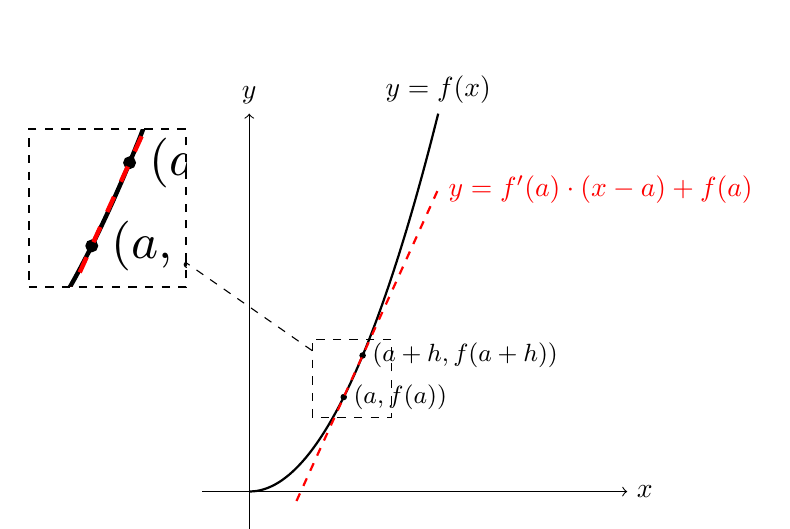
\begin{tikzpicture}[scale=1.2,  spy using outlines={rectangle, magnification=2, size=2cm, connect spies}]
        \draw[->] (-0.5,0) -- (4,0) node[right] {$x$};
        \draw[->] (0,-0.5) -- (0,4) node[above] {$y$};
        \draw[fill=black] (1,1) circle (.8pt) node[right](.5pt) {\small $(a, f(a))$};
        \draw[fill=black] (1.2,1.44) circle (.8pt) node[right] {\small $(a+h, f(a+h))$};
        
        \draw[domain=0:2, smooth, thick] plot (\x,\x*\x) node[above]{$y=f(x)$};
        \draw[domain=.5:2, smooth, thick, dashed, red] plot (\x,2.2*\x-1.2) node[right]{$y=f'(a)\cdot (x-a)+f(a)$};

        \spy [black, dashed] on (1.3, 1.44) in node at (-1.5,3);
    \end{tikzpicture}
\end{center}
\subsection{Symbols for the Derivative}
\[
    D_xf\text{, }
    \frac{d}{dx}f(x)\text{, }
    y'\text{, }
    \dot{y}
\]

\section{Rules and Derivatives of Elementary Functions}
\subsection{Derivative Rules}
\begin{enumerate}
    \item Constant Rule:
    $\displaystyle
        \frac{d}{dx}c = 0
    $
    
    \item Power Rule:
    $\displaystyle
        \frac{d}{dx}x^n = nx^{n-1}
    $
    
    \item Sum/Difference Rule:
    $\displaystyle
        \frac{d}{dx}[f \pm g] = \frac{d}{dx}f \pm \frac{d}{dx}g
    $
    
    \item Product Rule:
    $\displaystyle
        \frac{d}{dx}[f \cdot g] = \frac{d}{dx}f \cdot g + f \cdot \frac{d}{dx}g
    $
    
    \item Quotient Rule:
    $\displaystyle
        \frac{d}{dx}\left(\frac{f}{g}\right) = \frac{\frac{d}{dx}f \cdot g - f \cdot \frac{d}{dx}g}{g^2}
    $
\end{enumerate}
\subsection{Trigonometric Functions}
$
    \begin{array}{l@{\qquad}l}
        \qquad\frac{d}{dx}(\sin x) = \cos x & \displaystyle \frac{d}{dx}(\cos x) = -\sin x \\[10pt]
        \qquad\displaystyle \frac{d}{dx}(\tan x) = \sec^2 x & \displaystyle \frac{d}{dx}(\cot x) = -\csc^2 x \\[10pt]
        \qquad\displaystyle \frac{d}{dx}(\sec x) = \sec x \tan x & \displaystyle \frac{d}{dx}(\csc x) = -\csc x \cot x \\
    \end{array}
$
\subsection{Inverse Trigonometric Functions}
$
    \begin{array}{l@{\qquad}l}
        \qquad\displaystyle \frac{d}{dx}(\sin^{-1} x) = \frac{1}{\sqrt{1 - x^2}} 
        & \displaystyle \frac{d}{dx}(\cos^{-1} x) = \frac{-1}{\sqrt{1 - x^2}} \\[10pt]
        \qquad\displaystyle \frac{d}{dx}(\tan^{-1} x) = \frac{1}{1 + x^2} 
        & \displaystyle \frac{d}{dx}(\cot^{-1} x) = \frac{-1}{1 + x^2} \\[10pt]
        \qquad\displaystyle \frac{d}{dx}(\sec^{-1} x) = \frac{1}{|x|\sqrt{x^2 - 1}} 
        & \displaystyle \frac{d}{dx}(\csc^{-1} x) = \frac{-1}{|x|\sqrt{x^2 - 1}}
    \end{array}
$
\subsection{Exponential and Logarithhmic Functions}
$
    \begin{array}{l@{\qquad}l}
        \qquad\displaystyle \frac{d}{dx}(e^x) = e^x, & \displaystyle \frac{d}{dx}(\ln x) = \frac{1}{x},\,x>0\\[10pt]
        \qquad\displaystyle \frac{d}{dx}(a^x) = a^x \ln a,\,a>0 \,\&\,\neq 1 \quad & \displaystyle \frac{d}{dx}(\log_a x) = \frac{1}{x \ln a},\,a>0 \,\&\,\neq 1
    \end{array}
$
\subsection{Derivative of Inverse Function}
Let $f$ be a one-to-one differentiable function with inverse $f^{-1}$, and suppose $f'(f^{-1}(x)) \neq 0$. \\Then,
\[
    \left(f^{-1}\right)'(x) = \frac{1}{f'\left(f^{-1}(x)\right)}
\]
\subsubsection*{Example:} Let $f(x) = e^x$, so $f^{-1}(x) = \ln x$. Then,
\[
    \frac{d}{dx}(\ln x) = \frac{1}{\frac{d}{dx}(e^x)|_{x = \ln x}} = \frac{1}{e^{\ln x}} = \frac{1}{x}
\]
\subsection{Chain Rule}
If $h(x) = f(g(x))$ where both $f$ and $g$ are differentiable, then
\[
    h'(x) = \frac{d}{dx} f(g(x)) = f'(g(x)) \cdot g'(x).
\]

\section{Advanced Differentiation}
\subsection{Implicit Differentiation}
If a function $y$ is given implicitly by an equation involving both $x$ and $y$, such as
\[
    F(x,y) = 0.
\]
To find the derivative $\displaystyle\frac{dy}{dx}$, we differentiate both sides of the equation with respect to $x$, treating $y$ as a function of $x$.
\subsubsection*{Example:} If
\[
    x^2 + y^2 = 25,
\]
then differentiating both sides gives
\[
    2x + 2y \frac{dy}{dx} = 0.
\]
Solving for $\displaystyle\frac{dy}{dx}$ gives
\[
    \frac{dy}{dx} = -\frac{x}{y}.
\]
\subsection{Higher-Order Derivatives}
The second derivative, third derivative, and beyond are called higher-order derivatives. 
These describe how the rate of change itself changes.
\[
    \begin{cases}
    \displaystyle
        \frac{dy}{dx}, \,
        \frac{d^2y}{dx^2}, \, 
        \frac{d^n y}{dx^n}\\
        f'(x), \, f''(x), \, f'''(x), \, f^{(n)}(x)\\
        \dot{y}, \, \ddot{y}, \, \overset{...}{y}
    \end{cases}
\]
\subsection{Derivative of Parametric Functions}
Given a parametric curve:
\[
    x=x(t)\quad y=y(t)
\]
the derivative of $y$ w.r.t $x$ is given by
\[
    \frac{dy}{dx}=\frac{dy}{dt}\cdot\frac{dt}{dx}\quad \text{(provided } \frac{dx}{dt} \neq 0\text{)}
\]
\subsection{Derivative of Polar Functions}
For polar representations, $r=f(x)$ and that $x=r\cdot\cos\theta, \,y=r\sin\theta$.
\begin{align*}
    \frac{dx}{d\theta}=\frac{dr}{d\theta}\cdot\cos\theta - r\sin\theta\\[.5em]
    \frac{dy}{d\theta}=\frac{dr}{d\theta}\cdot\sin\theta + r\cos\theta
\end{align*} 
Thus,
\[
    \frac{dy}{dx}=\frac{dy}{d\theta}\cdot\frac{d\theta}{dx}=\frac{\frac{dr}{d\theta}\cdot\sin\theta + r\cos\theta}{\frac{dr}{d\theta}\cdot\cos\theta - r\sin\theta}
\]
\subsection{Derivative of Vector-valued Function}
Assume the position of a particle is given by $r=\left<x,y\right>$, it's velocity vector is given by 
\[
    \frac{dr}{dt}=\left<\frac{dx}{dt}, \frac{dy}{dt}\right>
\]
and the magnitude \textbf{speed} is thus
\[
    \left|\left|\frac{dr}{dt}\right|\right|=\sqrt{{\left(\frac{dx}{dt}\right)}^2+ {\left(\frac{dy}{dt}\right)}^2}
\]
Similarily, acceleration vector is
\[
    \frac{d^2r}{{dt}^2}=\left<\frac{d^2x}{{dt}^2}, \frac{d^2y}{{dt}^2}\right>
\]    
and the magnitude of acceleration is
\[
    \left|\left|\frac{d^2r}{{dt}^2}\right|\right|=\sqrt{{\left(\frac{d^2x}{{dt}^2}\right)}^2+ {\left(\frac{d^2y}{{dt}^2}\right)}^2}
\]

\section{Theorems}
\subsection{Rolle's Theorem}
Let $f$ be continuous on $[a, b]$, differentiable on $(a, b)$, and $f(a) = f(b)$.  
Then there exists $c \in (a, b)$ such that
\[
    f'(c) = 0.
\]
\begin{center}
    \begin{tikzpicture}[scale=1.2]
        \draw[->] (-0.5,0) -- (4.5,0) node[right] {$x$};
        \draw[->] (0,-2) -- (0,2) node[above] {$y$};

        \draw[domain=.5:3.5, smooth, thick] plot (\x,{(\x-1)*(\x-3)}) node[above right] {$f(x)$};
        \draw[fill=black] (1,0) circle (1pt) node[below left] {\small $a$};
        \draw[fill=black] (3,0) circle (1pt) node[below right] {\small $b$};
        \draw[dashed, thick, domain=1:3] plot (\x,-1) node[right] {$y = f'(c)(x - c) + f(c)$};
        \fill (2,-1) circle (1pt) node[below] {$c$};
    \end{tikzpicture}
\end{center}
\subsection{Mean Value Theorem}
If $f$ is continuous on $[a, b]$ and differentiable on $(a, b)$, then  
there exists $c \in (a, b)$ such that
\[
    f'(c) = \frac{f(b) - f(a)}{b - a}.
\]
\begin{center}
    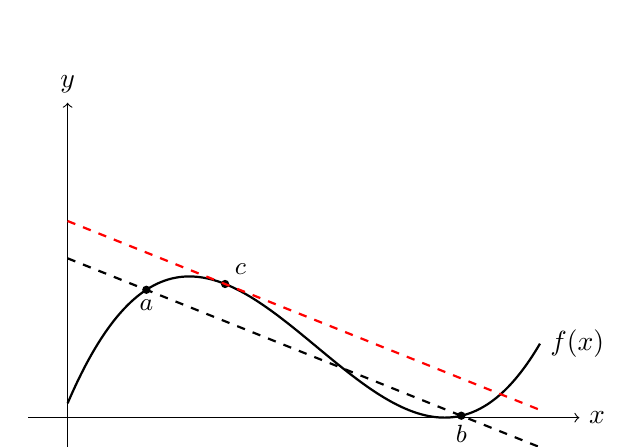
\begin{tikzpicture}[scale=1.0]
        \draw[->] (-0.5,0) -- (6.5,0) node[right] {$x$};
        \draw[->] (0,-0.5) -- (0,4) node[above] {$y$};

        \def\A{0.10526315789473684}
        \def\B{-1}
        \def\C{2.3368421052631579}
        \def\D{0.18197226735442307}

        \def\fone{1.6240775305123178}
        \def\ftwo{1.6977617410386339}
        \def\ffive{0.02407753051231865}
        \def\xmin{4.787708855438377}

        \draw[domain=0:6, samples=240, smooth, thick]
            plot (\x, {\A*(\x)^3 + \B*(\x)^2 + \C*(\x) + \D}) node[right] {$f(x)$};

        \coordinate (Apt) at (1, {\A*1^3 + \B*1^2 + \C*1 + \D});
        \coordinate (Bpt) at (5, {\A*125 + \B*25 + \C*5 + \D});
        \fill (Apt) circle (1.5pt) node[below] {\small $a$};
        \fill (Bpt) circle (1.5pt) node[below] {\small $b$};

        \def\m{-0.4}
        \draw[dashed, thick]
            plot[domain=0:6] (\x, {\m*(\x-1) + \fone});

        \coordinate (Cpt) at (2, {\A*8 + \B*4 + \C*2 + \D});
        \fill (Cpt) circle (1.5pt) node[above right] {\small $c$};
        \draw[dashed, thick, red]
            plot[domain=0:6] (\x, {\m*(\x-2) + \ftwo});

    \end{tikzpicture}
\end{center}
\subsection{Cauchy's Mean Value Theorem}
Let $f$ and $g$ be functions continuous on the closed interval $[a, b]$, and differentiable on the open interval $(a, b)$, with $g'(x) \ne 0$ for all $x \in (a, b)$. Then there exists at least one point $c \in (a, b)$ such that:
\[
    \frac{f'(c)}{g'(c)} = \frac{f(b) - f(a)}{g(b) - g(a)}
\]
For $g(x)=x$, Cauchy's Mean Value Theorem reduces to Mean Value Theorem. 
\subsection{Extreme Value Theorem}
If $f$ is continuous on $[a, b]$, then there exist points $c, d \in [a, b]$ such that
\[
    f(c) \leq f(x) \leq f(d) ,\quad \forall x \in [a, b].
\]
\begin{center}
    \begin{tikzpicture}[scale=1.0]
        \draw[->] (-0.5,0) -- (6.5,0) node[right] {$x$};
        \draw[->] (0,-2.5) -- (0,2.5) node[above] {$y$};

        \draw[domain=0:6, samples=200, smooth, thick]
            plot (\x, {2*sin(deg(pi*\x/3))}) node[above right] {$f(x)$};

        \coordinate (A) at (0, {2*sin(deg(0))});
        \coordinate (B) at (6, {2*sin(deg(pi))});
        \fill (A) circle (1.5pt) node[below left] {\small $a$};
        \fill (B) circle (1.5pt) node[below right] {\small $b$};

        \coordinate (c) at (1.5, {2*sin(deg(pi/2))});
        \fill (c) circle (1.5pt) node[above] {\small $c$ max };

        \coordinate (d) at (4.5, {2*sin(deg(pi/2*3))});
        \fill (d) circle (1.5pt) node[above] {\small $d$};
        \draw[dashed, gray] (1.5,0) -- (1.5,2);
        \draw[dashed, gray] (4.5,0) -- (4.5,-2);

    \end{tikzpicture}
\end{center}

\section{Behavior of Functions}
\subsection{Critical Points and Extrema}
\begin{itemize}
    \item \textbf{Critical Point:} A point $c$ in the domain of $f$ where $f'(c) = 0$ or $f'(c)$ does not exist.
    \item \textbf{Local Maximum:} $f(c)$ is a local maximum if $f(c) \geq f(x)$ for all $x$ near $c$.
    \item \textbf{Local Minimum:} $f(c)$ is a local minimum if $f(c) \leq f(x)$ for all $x$ near $c$.
\end{itemize}
\begin{center}
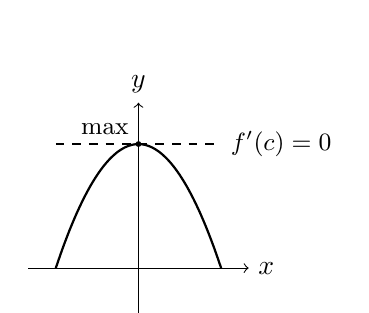
\begin{tikzpicture}[scale=0.7]
    \draw[->] (-2,0) -- (2,0) node[right] {$x$};
    \draw[->] (0,-1) -- (0,3) node[above] {$y$};
    \draw[domain=-1.5:1.5,smooth, thick] plot(\x,{ -(\x)^2 + 2.25});
    \draw[domain=-1.5:1.5,smooth, dashed] plot(\x,{2.25}) node [right]{\small $f'(c)=0$};
    \fill (0,2.25) circle (1.5pt) node[above left] {\small max};
\end{tikzpicture}
\hspace{1cm}
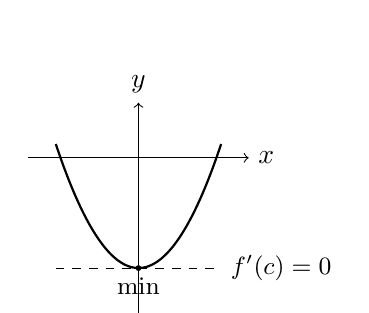
\begin{tikzpicture}[scale=0.7]
    \draw[->] (-2,0) -- (2,0) node [right] {$x$};
    \draw[->] (0,-3) -- (0,1) node [above] {$y$};
    \draw[domain=-1.5:1.5,smooth, thick] plot(\x,{ (\x)^2 - 2});
    \draw[domain=-1.5:1.5,smooth, dashed] plot(\x,-2) node [right]{\small $f'(c)=0$};
    \fill (0,-2) circle (1.5pt) node [below] {\small min};
\end{tikzpicture}
\end{center}
\subsection{Concavity and Inflection Points}
\begin{itemize}
    \item \textbf{Concave Up:} $f''(x) > 0$ on an interval $\implies$ graph lies above tangent lines.
    \item \textbf{Concave Down:} $f''(x) < 0$ on an interval $\implies$ graph lies below tangent lines.
    \item \textbf{Inflection Point:} A point where $f''(x)$ changes sign.
\end{itemize}
\begin{center}
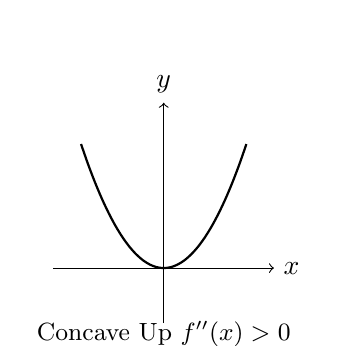
\begin{tikzpicture}[scale=0.7]
    \draw[->] (-2,0) -- (2,0) node [right] {$x$};
    \draw[->] (0,-1) -- (0,3) node [above] {$y$};
    \draw[domain=-1.5:1.5,smooth,thick] plot(\x,{ (\x)^2 });
    \node at (0,-1.2) {\small Concave Up $f''(x)>0$};
\end{tikzpicture}
\hspace{1cm}
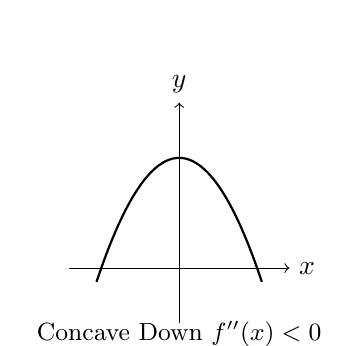
\begin{tikzpicture}[scale=0.7]
    \draw[->] (-2,0) -- (2,0) node [right] {$x$};
    \draw[->] (0,-1) -- (0,3) node [above] {$y$};
    \draw[domain=-1.5:1.5,smooth,thick] plot(\x,{ -(\x)^2 + 2});
    \node at (0,-1.2) {\small Concave Down $f''(x)<0$};
\end{tikzpicture}
\hspace{1cm}
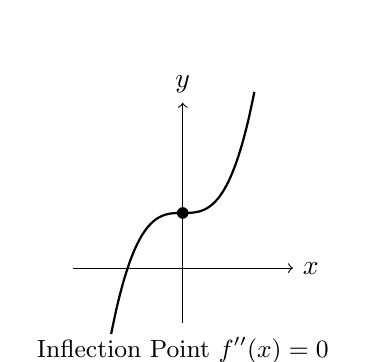
\begin{tikzpicture}[scale=0.7]
    \draw[->] (-2,0) -- (2,0) node [right] {$x$};
    \draw[->] (0,-1) -- (0,3) node [above] {$y$};
    \draw[domain=-1.3:1.3,smooth,thick] plot (\x, {(\x)^3+1});
    \fill (0,1)circle (3pt);
    \node at (0,-1.5) {\small Inflection Point $f''(x)=0$};
\end{tikzpicture}
\end{center}

\section{Applications}
\subsection{Related Rates}
\subsubsection{Angle of Elevation Problem}
A camera on the ground 200 meters away from a hot air balloon, also on the ground, records the balloon rising into the sky at a constant rate of 10 m/sec. How fast is the camera's angle of elevation changing when the balloon is 150m in the air? 
\begin{center}
    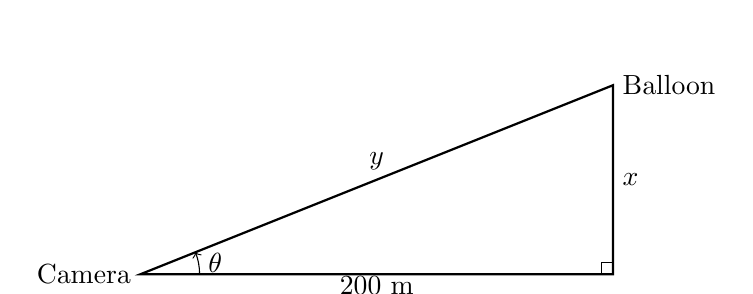
\begin{tikzpicture}[scale=0.03]

    \coordinate (C) at (0,0,0);
    \coordinate (A) at (200,0,0);
    \coordinate (B) at (200,80,0);

    \draw[thick] (C) -- (A) -- (B) -- cycle;

    \draw (200,0,0) -- ++(-5,0,0) -- ++(0,5,0) -- ++(5,0,0);

    \node at (100,-5,0) {200 m};
    \node[left] at (C) {Camera};
    \node[right] at (B) {Balloon};
    \node[above] at (100,40,0) {$y$};
    \node[right] at (200,40,0) {$x$};
    \tdplotdrawarc[->]{(C)}{25}{0}{21.8}{anchor=west}{$\theta$}

    \end{tikzpicture}
\end{center}
\subsubsection*{Solution}
Given $\displaystyle\frac{dx}{dt}=10$ m/sec and $\displaystyle\tan\theta = \frac{x}{200}$, we want $\displaystyle\frac{d\theta}{dt}$ at $x=150$. We differentiate both sides with respect to $t$. 
\[
    \begin{split}
        &\frac{d}{dt}\left(\tan\theta = \frac{x}{200}\right)\\[.5em]
        \Rightarrow&\sec^2\theta\frac{d\theta}{dt}=\frac{1}{200}\frac{dx}{dt}\\[.5em]
        \Rightarrow&\frac{d\theta}{dt}=\left.\frac{1}{200\sec^2\theta}\frac{dx}{dt}\right|_{\frac{dx}{dt}=10}=\frac{1}{20}\cos^2\theta
    \end{split}
\]
We have $\displaystyle\frac{d\theta}{dt}=\frac{1}{20}\cos^2\theta$, and at $x=150$, $y=250$ (by Pythagorean Theorem: $y^2=150^2+200^2$).
Thus, 
\[
    \begin{split}
        \left.\frac{d\theta}{dt}\right|_{x=150}&=\frac{1}{20}\cos^2\theta\\[.5em]
        &=\frac{1}{20}\left(\frac{4}{5}\right)^2\\[.5em]
        &=\frac{4}{125}= .032 
    \end{split}
\]
Thus, the angle of elevation changes at $.032$ radian/sec when the balloon is $150$m in the air.
\subsubsection{Inverted Cone (Water Tank) Problem}
\subsection{Optimization Problems}
\subsubsection{Area Problem}
The graph of $\displaystyle y=-\frac{1}{2}x+2$ encloses a region with the x-axis and y-axis in the first quadrant. A rectangle in the enclosed region has a vertex at the origin and the opposite vertex on the graph of $y$. Find the dimensions of the rectangle so that its area is a maximum. 
\begin{center}
\begin{tikzpicture}[scale=0.8]
    \draw[->] (-1,0) -- (8,0) node[right] {$x$};
    \draw[->] (0,-1) -- (0,4) node[above] {$y$};

    \coordinate (P) at (2,1);
    \draw[thick,domain=-1:6,samples=100] plot (\x,{-.5*\x + 2}) node[right]{$\displaystyle y=-\frac{1}{2}x+2$};
    \fill (P) circle (2pt) node[above right] {$P(x, y)$};
    \draw[dashed] (2,0)--(P)--(0,1);
\end{tikzpicture}
\end{center}


\subsubsection{Shortest Distance Problem}
Find the shortest distance between the point $(19, 0)$ and the parabola $y=(x-1)^2$.
\begin{center}
\begin{tikzpicture}[scale=0.4]
    \draw[->] (-1,0) -- (21,0) node[right] {$x$};
    \draw[->] (0,-1) -- (0,10) node[above] {$y$};

    \draw[thick,domain=-1:4,samples=100] plot (\x,{(\x-1)^2});

    \fill (19,0) circle (2pt) node[below right] {$A(19,0)$};

    \coordinate (P) at (3, 4);
    \fill (P) circle (3pt);
    \draw[dashed] (19,0) -- (P);
    \node[above] at (5, 4) {$(x_0, y_0)$};
\end{tikzpicture}
\end{center}
\subsubsection*{Solution}
Let $D$ be the distance between the point and the parabola 
\[
    \begin{split}
        D&=\sqrt{(x-19)^2+(y-0)^2}\\[.5em]
        &=\sqrt{(x-19)^2+((x-1)^2-0)^2}\\[.5em]
    \end{split}    
\]
To simplify the calculation, we consider $L=D^2$: 
\[
    L=D^2=(x-19)^2+(x-1)^4
\]
Differentiate $L$:
\[
    \begin{split}
        \frac{dL}{dx}&=\frac{d}{dx}\left((x-19)^2+(x-1)^4\right)\\[.5em]
        &=2(x-19)+4(x-1)^3
    \end{split}
\]
Set $L=0$:
\[
    \begin{split}
        \frac{dL}{dx}&=2(x-19)+4(x-1)^3\\[.5em]
        &=(x-3)(2x^2+7)\\[.5em]
        \Rightarrow &\,x=3
    \end{split}
\]
Apply the First Derivative Test:
\begin{center}
    \begin{tikzpicture}[scale=1]
        \draw[->] (-1,0) -- (6,0);

        \draw (0,0.15) -- (0,-0.15) node[below] {$0$};
        \draw (3,0.15) -- (3,-0.15) node[below] {$3$};
        
        \node[above] at (-1.5, .5) {$L'$};
        \node[above] at (-1.5, -1) {$L$};
        \node[above] at (1.5, .5) {$-$};
        \node[above] at (4.5, .5) {$+$};
        \node[above] at (3, .5) {$0$};
        \node[above] at (1.5, -1) {$decr.$};
        \node[above] at (4.5, -1) {$incr.$};

        \draw[->] (3, -1)--(3, -1.5) node[below]{$min.$};
    \end{tikzpicture}
\end{center}
Since $x=3$ is the only relative min point, it is the absolute min.\\ 
Thus, the shortest distance is
\[
    \left.D\right|_{x=3}=\sqrt{(3-19)^2+(3-1)^4}=4\sqrt{17}
\]
\subsection{Linear Approximation (First-Order Taylor Expantion)}
If $f$ is differentiable at $x=a$, then near $a$, the function $f(x)$ is approximated by
\[
    f(x) \approx f(a)+f'(a)(x-a)
\]
\subsubsection*{Example:}
for $x$ near $0$, $\sin x$ can be approximated by $\sin x \approx \sin(0) + \cos(0)\cdot x = x$
\begin{center}
    \begin{tikzpicture}[scale=2, spy using outlines={rectangle, magnification=1, size=1cm, connect spies}]
        \draw[->] (-1.7,0) -- (1.7,0) node[right] {$x$};
        \draw[->] (0,-1.2) -- (0,1.2) node[above] {$y$};

        \draw[domain=-1.5:1.5, smooth, thick, black] plot (\x, {sin(deg(\x))}) node[right]{$y=\sin x$} ;
        \draw[domain=-1.2:1.2, dashed, thick, red] plot (\x, \x) node[right]{$y=x$};

        \spy [black, dashed] on (0,{sin(deg(0))}) in node at (-1.5,1);
    \end{tikzpicture}
\end{center}
\end{document}